%% 
%% Template article for cas-sc documentclass for 
%% double column output.

\documentclass[a4paper,fleqn]{cas-sc}

% If the frontmatter runs over more than one page
% Use the longmktitle option.

%\documentclass[a4paper,fleqn,longmktitle]{cas-sc}

%\usepackage[numbers]{natbib}
%\usepackage[authoryear]{natbib}
\usepackage[numbers]{natbib}
%% The amssymb package provides various useful mathematical symbols
\usepackage{amssymb}
%% The amsmath package provides various useful equation environments.
\usepackage{amsmath}
\usepackage{epstopdf}
\usepackage{mathptmx,mathtools}
\usepackage{subcaption}
\usepackage{float} % Add this in your preamble
\usepackage[export]{adjustbox}
\usepackage{array} % Needed for m{} column type
\usepackage[percent]{overpic} % <-- put this in your preamble



\usepackage{amsmath}
\usepackage{nicefrac}
\usepackage{dirtytalk}
\usepackage{graphicx}   % For including images
\usepackage{tikz}
\usetikzlibrary{calc,tikzmark} % needed <<<<<<<<<<
\usepackage{xcolor}     % For coloring
\usepackage{lineno}
\renewcommand\linenumberfont{\normalfont\bfseries\small} % <-- Increase line number size
\usetikzlibrary{arrows.meta}
\usetikzlibrary{calc, positioning}
%%%Author macros
\def\tsc#1{\csdef{#1}{\textsc{\lowercase{#1}}\xspace}}
\tsc{WGM}
\tsc{QE}

\begin{document}
	
	\setcounter{figure}{1}
			\begin{figure}[!t]
		\centering
		
		% -------- Subfigure (a–g on one strip) -------- %
		\begin{subfigure}[t]{1\textwidth}
			\centering
			\begin{overpic}[width=\textwidth,trim={6.2cm 0cm 6.1cm 5cm},clip]{Fig5.eps}
				% Panel labels (yours)
				\put(4,52){\fontfamily{ptm}\selectfont\textbf{(a)}}
				\put(18,52){\fontfamily{ptm}\selectfont\textbf{(b)}}
				\put(32,52){\fontfamily{ptm}\selectfont\textbf{(c)}}
				\put(46,52){\fontfamily{ptm}\selectfont\textbf{(d)}}
				\put(60,52){\fontfamily{ptm}\selectfont\textbf{(e)}}
				\put(74,52){\fontfamily{ptm}\selectfont\textbf{(f)}}
				\put(88,52){\fontfamily{ptm}\selectfont\textbf{(g)}}
				
				% ======= CIRCULAR MAGNIFIED INSET (edit coordinates as needed) =======
				% Choose the center of the region to magnify (percent coordinates of overpic)
				
				\put(82.7,5.2){% <-- circle center on the main image
					\begin{tikzpicture}[overlay,remember picture]
						\def\rad{1.5mm}
						\draw[line width=0.8pt, black] (-0.9mm,0) circle (\rad);
						\draw[-{Triangle[length=2mm, width=2mm]}, line width=0.8pt, black]
						(0,0) -| (0.5,0.5)
						node[pos=1, above, font=\fontsize{6.5}{6.5}\fontfamily{ptm}\selectfont\bfseries]{Vortex core};
					\end{tikzpicture}
				}
				
				
				\put(22,5.2){% <-- circle center on the main image
					\begin{tikzpicture}[overlay,remember picture]
						\def\rad{1.5mm}
						\draw[line width=0.8pt, black] (-0.4mm,-0.1mm) circle (\rad);
						\draw[-{Triangle[length=2mm, width=2mm]}, line width=0.8pt, black]
						(-2mm,0) -| (-0.5,0.5)
						node[pos=1, above, font=\fontsize{6.5}{6.5}\fontfamily{ptm}\selectfont\bfseries]{External flow};
					\end{tikzpicture}
				}
				
				
				\put(55,5.2){% <-- circle center on the main image
					\begin{tikzpicture}[overlay,remember picture]
						\def\rad{1.5mm}
						\draw[line width=0.8pt, black] (0mm,0) circle (\rad);
						\draw[-{Triangle[length=1.5mm, width=1.5mm]}, line width=0.8pt, black]
						(0,1.3mm) |- (0.5,0.5)
						node[pos=1, right, font=\fontsize{6.5}{6.5}\fontfamily{ptm}\selectfont\bfseries]{Inside the wake};
						
						\draw[-{Triangle[length=1.5mm, width=1.5mm]}, line width=0.8pt, black]
						(0,-7mm) -- (4.5,-7mm)
						node[pos=1, right, font=\fontsize{6.5}{6.5}\fontfamily{ptm}\selectfont\bfseries]{Toward vortex};
						
					\end{tikzpicture}
				}
				
				
				\put(52,5.2){% <-- circle center on the main image
					\begin{tikzpicture}[overlay,remember picture]
						\def\rad{1.5mm}
						\draw[line width=0.8pt, black] (0mm,0) circle (\rad);
						\draw[-{Triangle[length=1.5mm, width=1.5mm]}, line width=0.8pt, black]
						(0,1.3mm) |- (-0.5,0.5)
						node[pos=1, left, font=\fontsize{6.5}{6.5}\fontfamily{ptm}\selectfont\bfseries]{Entrained};
						
						\draw[-{Triangle[length=1.5mm, width=1.5mm]}, line width=0.8pt, black]
						(-10mm,-7mm) -- (-4.5,-7mm)
						node[pos=1, left, font=\fontsize{6.5}{6.5}\fontfamily{ptm}\selectfont\bfseries]{Toward external flow};
						
					\end{tikzpicture}
				}
				
				\put(46,5.2){% <-- circle center on the main image
					\begin{tikzpicture}[overlay,remember picture]
						\def\rad{1.5mm}
						\draw[line width=0.8pt, black] (0mm,0) circle (\rad);
						\draw[-{Triangle[length=1.5mm, width=1.5mm]}, line width=0.8pt, black]
						(0,-1.3mm) |- (-0.5,-0.5)
						node[pos=1, left, font=\fontsize{6.5}{6.5}\fontfamily{ptm}\selectfont\bfseries]{Transition};
						
					\end{tikzpicture}
				}
				
				
				% ======= CIRCULAR MAGNIFIED INSET (edit coordinates as needed) =======
				% Choose the center of the region to magnify (percent coordinates of overpic)
				% Example: a small area near panel (d)
				%				\put(82,4.6){% <-- circle center on the main image
					%					\begin{tikzpicture}[overlay,remember picture]
						%						% radius in overpic "percent" roughly maps to textwidth; adjust by trial
						%						\def\rad{1.5mm}
						%						
						%						% Draw the circle on the main figure to indicate the zoom region
						%						\draw[line width=0.8pt, black] (-0.9mm,0) circle (\rad);
						%						
						%						% Place the circular inset at some offset (adjust xshift/yshift)
						%						\begin{scope}[shift={(3.8cm,1.2cm)}] % inset position relative to the circle marker
							%							% Clip to a circle
							%							\clip (0,0) circle (1.5*\rad);
							%							% Re-insert the SAME image, but cropped around the target area.
							%							% Tweak 'trim' to center the desired content inside the circle.
							%							\node[inner sep=0pt,anchor=center] at (0,0) {%
								%								\includegraphics[width=0.28\textwidth,
								%								clip,
								%								trim={25cm 4.0cm 10.5cm 7.5cm}]{Fig6.eps}};
							%						\end{scope}
						%						
						%						% Draw the visible circular border of the inset
						%						%\draw[line width=0.8pt, ] ([shift={(3.8cm,1.2cm)}]0,0) circle (1.5*\rad);
						%						
						%						% Connector line from the marked circle to the inset
						%						\draw[-{Triangle[length=2mm, width=2mm]}, line width=0.8pt, black]
						%						(0,0) -- ([shift={(1cm,0cm)}]0,0);
						%						
						%					\end{tikzpicture}
					%				}
				
				% ======= END INSET =======
			\end{overpic}
		\end{subfigure}%
		
		\caption{Temporal backward (a–c) and forward (e–g) evolution of the wake and its influence on the surrounding flow regions around the rising bubble for case $C_6$. The flow regions are separated by the hyperbolic LCSs obtained from the forward FTLE field with $\Delta\tau = 10$ at $\tau = 3.6$, as shown in (d), where the outermost and innermost structures are indicated by red and blue solid lines, respectively. The corresponding elliptic LCSs, shown in green with a color spectrum increasing toward the vortex core, highlight regions of rotational coherence. Panels (a–c) correspond to $\tau = 0.05$, $0.75$, and $2.0$, respectively, representing the backward evolution, while panels (e–g) correspond to $\tau = 5.4$, $7.0$, and $8.0$, showing the forward evolution. The light-blue regions represent the surrounding fluid, while the yellow and dark-blue regions denote the fluid above the bubble, with the dark-blue area located near the bubble top surface.}
		\label{Fig5}
	\end{figure}
	%%%%%%%%%%%%%%%%%%%%%%%%%%%%%________Figure_5___________%%%%%%%%%%%%%%%%%%%%%
	
\end{document}